\chapter{Marco Teórico}

\section{Realidad Virtual e interacción inmersiva}
La investigación sobre la realidad virtual (VR, 
por sus siglas en inglés) ha evolucionado más 
allá de solo buscar una experiencia tridimensional 
hacia la integración en las interacciones y la 
experiencia del usuario. Las aplicaciones 
inmersivas actuales no dependen únicamente de la 
calidad gráfica del entorno, sino también de la 
correspondencia entre las acciones físicas 
realizadas por el usuario, las respuestas 
producidas por el sistema y los mecanismos 
mediante los cuales se comunican los resultados 
de cada interacción \cite{chen2024interfaces,spittle2023interaction,yeo2024interfaces}.
Como consecuencia, el diseño de experiencias de 
VR abarca un campo interdisciplinario en el que 
se unen aspectos computacionales, perceptuales y 
ergonómicos.

Las interfaces de interacción en VR ocupan 
diferentes mecanismos de entrada, seguimiento y 
retroalimentación, entre ellos controladores, 
seguimiento de manos, reconocimiento de gestos y 
dispositivos hápticos \cite{chen2024interfaces}. 
Por ello, la incorporación de una tecnología de 
entrada no garantiza por sí sola una interacción 
adecuada, sino que debe responder a las tareas 
que forman parte de la experiencia. Las técnicas 
de interacción empleadas en entornos inmersivos 
pueden organizarse de acuerdo con tareas como la 
selección, la manipulación, la navegación y el 
control del sistema \cite{spittle2023interaction}.
No existe una técnica de interacción que resulte 
igualmente efectiva para todas las aplicaciones, 
pues su utilidad depende de las características 
de los objetos, la actividad realizada, el 
\textit{hardware} disponible y el contexto de uso. 
Esta dependencia del contexto es especialmente 
relevante en experiencias gamificadas, donde una 
misma sesión puede incluir acciones diferentes 
como apuntar, alcanzar, desplazarse o activar 
elementos virtuales.

Durante las primeras investigaciones sobre 
interfaces tridimensionales también se demostró 
que una interacción técnicamente funcional no 
necesariamente produce una experiencia 
comprensible o satisfactoria \cite{yeo2024interfaces}.
Las técnicas de selección y manipulación deben 
proporcionar señales que permitan reconocer qué 
objetos pueden utilizarse, cuando se ha detectado 
una acción y cuál ha sido su resultado \cite{chen2024interfaces}.
En consecuencia, la claridad de una interacción 
depende tanto de la entrada ejecutada por el 
usuario como de la respuesta inmediata que el 
sistema genera.

La retroalimentación visual y háptica ha sido 
investigada como un medio para comunicar el 
estado de los objetos y confirmar el resultado de 
las acciones dentro de entornos virtuales \cite{chen2024interfaces,gibbs2022feedback}.
La combinación de diferentes canales sensoriales puede contribuir a que 
el usuario perciba una relación más clara entre sus movimientos físicos 
y los acontecimientos del entorno virtual. La retroalimentación 
multisensorial no debe considerarse únicamente como un componente 
estético, sino como una parte funcional de la interfaz que permite 
informar sobre aciertos, errores, contacto con objetos y cambios en el 
estado del sistema.

Además de la interacción, también se ha estudiado dimensiones como la 
presencia, la experiencia de usuario y el \textit{cybersickness}. Estos 
elementos permiten examinar la calidad de una experiencia inmersiva más 
allá de su funcionamiento técnico \cite{wang2025presence,bareisyte2024questionnaires}.
La presencia se relaciona con la percepción de encontrarse dentro del 
entorno virtual, mientras que el \textit{cybersickness} trata de 
diferentes formas de malestar que pueden surgir durante el uso de 
dispositivos VR \cite{sepich2022workload}. Debido a que ambas 
dimensiones pueden estar influenciadas por el diseño de las tareas, la 
retroalimentación y la carga impuesta al usuario, resultan relevantes al 
analizar aplicaciones interactivas en VR \cite{gibbs2022feedback}.

La evaluación de experiencias de VR suele combinar información objetiva 
registrada por el sistema con información subjetiva proporcionada por 
los participantes \cite{wang2025presence,bareisyte2024questionnaires}.
Las métricas fisiológicas y conductuales pueden utilizarse para 
complementar la medición de presencia, aunque su interpretación depende 
del contexto y de las condiciones específicas de cada experiencia. De 
manera similar, existe una amplia variedad de cuestionarios orientados a 
evaluar presencia, usabilidad, experiencia de usuario y malestar, pero 
no todos utilizan las mismas definiciones ni miden exactamente los 
mismos componentes. Por esta razón, la selección de instrumentos y 
métricas debe responder a los objeticos concretos de cada investigación.

La carga generada por una tarea puede influir en el nivel de malestar 
experimentado por el usuario dentro de un entorno virtual \cite{sepich2022workload}.
Esto implica que la dificultad de una actividad inmersiva no debe 
evaluarse únicamente mediante tasas de éxito o fracaso. Una tarea 
excesivamente rápida, compleja o demandante también puede afectar la 
claridad de la interacción y el \textit{confort} del participante. La 
adaptación dentro de una aplicación inmersiva no puede plantearse 
únicamente como un mecanismo para aumentar o disminuir la dificultad, 
sino como una herramienta para mantener condiciones de interacción 
apropiadas para el comportamiento observado del usuario. Por ello, un 
sistemas adaptativos, debe modificar la dificultad tomando en cuenta 
como eso altera las exigencias que la experiencia impone al usuario.

\section{Videojuegos y experiencias musicales interactivas}
La relación entre música e interacción de videojuegos ha sido estudiada 
desde distintas formas de participación del jugador y de integración del 
sonido con las mecánicas. En particular, la literatura sobre 
interactividad en videojuegos musicales identifica principios mediante 
los cuales la música puede incorporarse a las reglas, acciones, 
estructuras temporales y mecanismos de respuesta de una experiencia 
interactiva \cite{pichlmair2007sound}. A partir de este enfoque, los 
videojuegos musicales pueden analizarse no únicamente por utilizar 
música como acompañamiento, sino por la forma en que los elementos 
musicales intervienen directamente en el \textit{gameplay}.

Existen múltiples maneras en las que se puede interactuar en un 
videojuego musical, como la ejecución de acciones rítmicas, el 
seguimiento de una estructura temporal, la asociación entre sonido y 
elementos visuales, la interpretación de secuencias y la modificación de 
componentes sonoros \cite{pichlmair2007sound}. Estas formas de interacción crean diferentes niveles 
de participación. En algunos casos, el usuario crea o modifica 
directamente el sonido, mientras que en otros ejecuta acciones que son 
evaluadas de acuerdo con que tanto se apeguen a una estructura musical 
establecida. 

La música también puede cumplir varias funciones dentro de una 
experiencia interactiva. Puede actuar como guía temporal, como 
respuesta a las acciones realizadas, como elemento que organiza la 
progresión o como parte central de las reglas del juego. Esto diferencia 
a las experiencias musicales interactivas de aquellas en las que una 
canción funciona únicamente como fondo sonoro. En una experiencia 
gamificada, la relación entre música y acción puede determinar cuándo 
debe intervenir el usuario, qué tipo de respuesta debe realizar y cómo 
se comunica el resultado de su participación \cite{rashed2025engagement}.

Lo anterior crea un reto para el desarrollador. Las exigencias del 
\textit{gameplay} deben permitir que el usuario participe activamente 
sin desplazar por completo su atención de la música y del entorno. 
Cuando las tareas requieren una concentración excesiva o presentan una 
dificultad inadecuada, la experiencia puede convertirse únicamente en 
una cadena de objetivos mecánicos \cite{rashed2025engagement}. Por el 
contrario, una actividad con muy poca exigencia puede reducir el 
involucramiento del jugador. La literatura sobre videojuegos musicales 
plantea, por tanto, la necesidad de conservar una relación coherente 
entre sonido, interacción, dificultad y respuesta del sistema.

\section{Adaptación dinámica y ajuste de dificultad}
La adaptación dinámica en videojuegos comprende enfoques en los que la 
información obtenida durante la interacción del jugador se utiliza para 
modificar distintos componentes de la experiencia. Las revisiones sobre 
adaptación basada en la experiencia describen este proceso como un ciclo 
en el que se observa al usuario, se interpreta su comportamiento y, 
posteriormente, se aplican cambios sobre elementos controlables del 
juego \cite{lopes2025closing}. Desde esta perspectiva, la adaptación 
busca reducir rigidez de experiencias que mantienen las mismas 
condiciones para todos los jugadores, permitiendo que el sistema 
responda a diferencias de desempeño y a cambios que ocurren durante una 
misma sesión.

Para completar este ciclo, la recopilación de información por sí sola no 
es suficiente. Las métricas registradas deben convertirse en una 
representación útil del jugador y, después, en decisiones capaces de 
modificar elementos concretos de la experiencia. La conexión entre 
medición, interpretación y modificación constituye uno de los aspectos 
centrales del diseño de sistemas adaptativos. En una experiencia musical 
interactiva, esta relación adquiere especial importancia porque los 
cambios deben responder al desempeño sin romper la coherencia entre 
\textit{gameplay}, interacción y experiencia musical \cite{pichlmair2007sound}.

Una de las formas más documentadas de adaptación es el ajuste dinámico 
de dificultad (DDA, por sus siglas en inglés). Este método modifica 
automáticamente características, comportamientos o escenarios de un 
videojuego durante su ejecución a partir de la habilidad o del desempeño 
observado en el jugador \cite{zohaib2018dda}. A diferencia de los niveles 
seleccionados antes de comenzar una partida, el ajuste dinámico puede 
responder a cambios ocurridos durante una misma sesión.

Los sistemas DDA pueden modificar parámetros como la velocidad, la 
cantidad de elementos, la disponibilidad de recursos, el comportamiento 
de los oponentes, la frecuencia de aparición de objetos y la complejidad 
de las tareas \cite{zohaib2018dda,huber2021dda}. En VR, también se ha 
investigado la generación y modificación de contenido con base en la 
experiencia del usuario, demostrando que la adaptación puede intervenir 
sobre la estructura de una actividad y no únicamente cambiar una 
etiqueta general de dificultad. La implementación de estos sistemas 
puede apoyarse en reglas heurísticas, modelos probabilísticos, 
redes neuronales, algoritmos evolutivos y otras técnicas de inteligencia 
computacional. No obstante, la utilización de modelos complejos no es un 
requisito para una solución adaptativa. Cuando el conjunto de métricas y 
parámetros está claramente delimitado, un sistema basado en reglas puede 
ofrecer cambios comprensibles, controlables y verificables durante el 
desarrollo. Un sistema adaptativo suele requerir un mecanismo que 
observe al jugador, una representación de su situación y un 
procedimiento que seleccione cambios en el videojuego. La observación 
puede realizarse mediante telemetría producida durante la partida. La 
representación puede consistir en valores numéricos, categorías o 
estados. Finalmente, el mecanismo de decisión determina qué parámetro 
debe modificarse, en qué magnitud y durante cuánto tiempo.

Los modelos temporales de jugador han demostrado que el desempeño no 
debe tratarse necesariamente como una característica estática \cite{zook2012temporal}.
Las capacidades observadas pueden cambiar conforme el usuario aprende 
las reglas, se acostumbra a los controles o enfrenta nuevas tareas. Por 
ello, un sistema de adaptación puede beneficiarse de analizar secuencias 
de interacciones y tendencias de desempeño, en lugar de reaccionar de 
manera inmediata ante cada acierto o error aislado.

La adaptación también ha sido estudiada como un procedimiento orientado 
a optimizar la satisfacción del jugador. Los modelos construidos a partir 
de características observables del juego pueden utilizarse para modificar 
parámetros controlables y mejorar la experiencia estimada durante la 
interacción \cite{yannakakis2009adaptation}. Este enfoque amplía el 
objetivo del ajuste, pues la modificación no busca únicamente facilitar 
o dificultar la tarea, sino aproximar la experiencia a una condición 
considerada apropiada para el usuario.

El DDA también se ha planteado como un mecanismo para sostener el 
involucramiento a lo largo de la sesión \cite{xue2017dda}. Desde esta 
perspectiva, la dificultad no se limita a un valor fijo, sino que puede 
representarse como una secuencia de estados y transiciones. El sistema 
decide cuándo aumentar, mantener o disminuir el desafío de acuerdo con 
la información registrada durante la partida. Esto permite considerar 
que los cambios deben producirse gradualmente y no como respuestas 
abruptas ante eventos individuales.

Los mecanismos de DDA requieren, además, evitar respuestas excesivamente 
sensibles a variaciones momentáneas del desempeño. Una modificación 
basada en eventos aislados puede generar oscilaciones frecuentes de 
dificultad, por lo que diferentes propuestas consideran tendencias 
temporales, límites de ajuste o periodos de observación antes de 
modificar nuevamente el \textit{gameplay} \cite{zook2012temporal,xue2017dda,zohaib2018dda}.
De esta manera, el ajuste dinámico no depende únicamente de qué 
parámetro modificar, sino también de determinar cuándo existe 
suficiente evidencia para aplicar el cambio.

\section{Métricas, modelado del jugador y ciclo de adaptación}
El funcionamiento de un sistema adaptativo depende de la información que 
pueda obtener del comportamiento del jugador y de la forma en que dicha 
información sea interpretada. La literatura sobre estimación del 
involucramiento utiliza telemetría, métricas de desempeño, patrones de 
interacción y, en algunos casos, señales fisiológicas como fuentes para 
caracterizar la experiencia del usuario \cite{rashed2025engagement}. A 
su vez, los enfoques de adaptación basada en experiencia señalan que 
estos datos adquieren utilidad cuando se incorporan a un modelo que 
permite relacionar el comportamiento observado con decisiones 
posteriores del sistema \cite{lopes2025closing}. En este sentido, las 
métricas y el modelado del jugador constituyen dos etapas conectadas 
dentro del ciclo de adaptación.

Entre las variables de desempeño empleadas en el modelado del jugador se 
encuentran los aciertos, errores, puntuaciones, tiempos de respuesta, 
duración de las acciones y frecuencia de interacción \cite{zook2012temporal,zohaib2018dda}.
Estas métricas no representan directamente estados psicológicos 
complejos, pero pueden funcionar como indicadores operativos del 
comportamiento observado. Su utilidad consiste en permitir que el 
sistema reconozca tendencias básicas, como un aumento sostenido de 
errores, una reducción en la frecuencia de respuestas o una mejora 
progresiva en la precisión. La frecuencia de interacción puede 
utilizarse para observar la continuidad de la participación y la 
relación entre aciertos y errores permite construir una medida básica de 
desempeño. Sin embargo, ninguna de estas variables debe interpretarse de 
forma aislada, debido a que un mismo resultado puede tener distintas 
explicaciones según la tarea y el momento de la experiencia.

En la estimación del involucramiento no existe una métrica única que 
represente completamente la experiencia del jugador. Los enfoques 
disponibles utilizan diferentes combinaciones de comportamiento, 
desempeño, telemetría y señales fisiológicas. Aunque estas últimas 
pueden proporcionar información adicional, también requieren equipo, 
procedimientos y formas de interpretación que incrementan la 
complejidad del sistema. Para prototipos de alcance delimitado, la 
telemetría generada directamente por el \textit{gameplay} representa 
una alternativa viable para implementar adaptación en tiempo real.

El modelado del jugador puede expresarse mediante variables continuas, 
perfiles, categorías o estados discretos. Los estados permiten resumir 
patrones de comportamiento y asociarlos con respuestas específicas del 
sistema. No obstante, deben entenderse como representaciones 
computacionales construidas a partir de reglas observables y no como 
diagnósticos del estado mental del usuario. Esta distinción es 
importante cuando se utilizan categorías como inactivo, interactuando, 
sobrecargado o en transición.

La literatura identifica una brecha entre la recolección de métricas, 
la interpretación de la información y la aplicación de cambios efectivos 
en el juego \cite{huber2021dda}. Algunos sistemas se concentran en medir 
al usuario, pero no utilizan los resultados para adaptar la experiencia. 
Otros modifican parámetros sin explicar claramente cómo se relacionan 
con el comportamiento observado. Para cerrar este ciclo, el sistema debe 
establecer relaciones explícitas entre las métricas registradas, los 
estados modelados y los parámetros que pueden modificarse.

Desde una perspectiva conceptual, estos elementos pueden organizarse 
como un ciclo de interacción y adaptación \cite{zohaib2018dda}. Primero, 
el usuario realiza acciones dentro del entorno virtual, luego el sistema 
registra métricas asociadas con dichas acciones y utiliza sus valores 
para construir una representación operativa de su comportamiento. Esta 
representación puede expresarse mediante estados discretos que 
sintetizan patrones recientes de interacción. Finalmente, el estado 
identificado y las métricas registradas sirven como entrada para 
determinar modificaciones sobre parámetros controlables del 
\textit{gameplay}, generando nuevas condiciones de interacción que 
vuelven a ser observadas por el sistema. De esta manera, la adaptación 
se plantea como un proceso continuo de observación, interpretación y 
respuesta, en lugar de como un cambio aislado de dificultad.

En conjunto, se identificó una progresión desde entornos virtuales que 
responden a entradas individuales hacia sistemas capaces de registrar 
patrones de comportamiento y modificar su funcionamiento durante la 
ejecución. Existen investigaciones sobre interfaces inmersivas, 
retroalimentación multisensorial, experiencias musicales, telemetría, 
modelado del jugador y ajuste dinámico de dificultad \cite{chen2024interfaces,spittle2023interaction,yeo2024interfaces,pichlmair2007sound,rashed2025engagement,lopes2025closing,zohaib2018dda,huber2021dda,wang2025presence,bareisyte2024questionnaires,sepich2022workload,gibbs2022feedback,yannakakis2009adaptation,zook2012temporal,xue2017dda}.
La relación entre estos conceptos permite comprender la adaptación como 
un ciclo continuo en el que las acciones del usuario generan información, 
la cuál es interpretada mediante un modelo y posteriormente se utiliza 
para modificar parámetros controlables de la experiencia \cite{lopes2025closing,rashed2025engagement,zohaib2018dda}.
Estos fundamentos proporcionan la base conceptual necesaria para el 
diseño del sistema de interacción adaptativa desarrollado en el 
presente trabajo.

\section{Métricas, modelado del jugador y ciclo de adaptación}
Una vez establecidos los fundamentos conceptuales que sustentan la 
interacción adaptativa, resulta necesario identificar las herramientas 
y tecnologías que permiten llevar estos principios a una implementación 
práctica dentro de una experiencia de VR. Una experiencia interactiva en 
VR requiere combinar herramientas orientadas al desarrollo de software,
creación de contenido tridimensional y comunicación con el dispositivo 
de realidad virtual. En este proyecto se utiliza Unity 6 como motor 
principal de desarrollo, Blender para la creación y modificación de 
recursos tridimensionales y herramientas de desarrollo proporcionadas 
por Meta para permitir la ejecución e interacción de la experiencia 
mediante los Meta Quest 2. Estas tecnologías cumplen funciones 
diferentes dentro del proceso, pero forman en conjunto el entorno 
técnico sobre el cual se implementará el sistema de interacción 
adaptativa.

\subsection{Unity 6}
Unity es un motor de desarrollo que permite construir aplicaciones 
interactivas en entornos bidimensionales y tridimensionales \cite{unity2024requirements}.
Su arquitectura integra herramientas para la administración de escenas, 
objetos, componentes, físicas, audio, animaciones, interfaces y 
programación de comportamientos, lo que permite centralizar dentro de 
un mismo entorno gran parte del proceso de desarrollo de una aplicación 
interactiva. Unity también cuenta con soporte para aplicaciones de 
realidad extendida (XR, por sus siglas en inglés) mediante una 
arquitectura basada en paquetes y complementos que permite integrar 
distintos dispositivos y plataformas XR.

Para el presente proyecto se utiliza Unity 6, correspondiente a la 
generación 6000 del motor. Esta versión contempla soporte para 
dispositivos XR autónomos, entre ellos Meta Quest 2. Dentro del 
ecosistema, el desarrollo de interacciones XR puede apoyarse en 
herramientas como XR \textit{Plug-in Management} y XR 
\textit{Interaction Toolkit}  \cite{unityxrmanagement,unityxrit}. 
La primera administra la inicialización, configuración y soporte de 
compilación de los complementos XR. Por su parte, la segunda 
proporciona un sistema de interacción basado en componentes para 
desarrollar experiencias de VR.

En el contexto de este trabajo, Unity funciona como la plataforma en la 
que se integrarán las mecánicas de los minijuegos, detección de 
interacciones, retroalimentación, registro de métricas, modelado de 
estados del jugador y reglas de adaptación dinámica. La elección de un 
motor con soporte específico para XR permite que estas funcionalidades 
puedan desarrollarse sobre una infraestructura de interacción existente, 
en lugar de implementar directamente las interfaces de bajo nivel 
requeridas para comunicarse con el dispositivo.

\subsection{Blender}
Blender es un conjunto de herramientas de creación tridimensional 
gratuito y de código abierto que cubre diferentes etapas de la 
producción de contenido digital, entre ellas modelado, texturizado, 
\textit{rigging}, animación, simulación y renderizado \cite{blenderfeatures}.
Además, puede utilizarse para la creación de recursos destinados a 
videojuegos y otras aplicaciones interactivas, lo que permite 
desarrollar ciertos elementos visuales en un entorno independiente antes 
de integrarlos en el motor. 

Para una experiencia ejecutada en un dispositivo de VR autónomo, la 
complejidad de los modelos tridimensionales es un factor relevante 
debido a las limitaciones de procesamiento del hardware. En este 
proyecto, esta herramienta permitirá elaborar y modificar a los 
personajes, objetos y elementos visuales asociados a los minijuegos 
antes de ser importados a Unity. El uso de una dirección visual 
estilizada y \textit{low-poly} permiten controlar la complejidad 
geométrica de estos recursos y mantener una apariencia visual coherente 
entre los diferentes elementos de la experiencia.

\subsection{Meta Quest 2 y herramientas de Meta XR}
Meta Quest 2 es un dispositivo autónomo de VR perteneciente a la familia 
Meta Quest. Este dispositivo integra visualización estereoscópica, 
seguimiento de la posición y orientación de la cabeza y mecanismos de 
entrada que permiten representar las acciones físicar del usuario dentro 
del entorno virtual. Unity 6 incluye los Quest 2 entre los dispositivos
XR autónomos soportados por su arquitectura de desarrollo.

\begin{figure}[H]
    \centering
    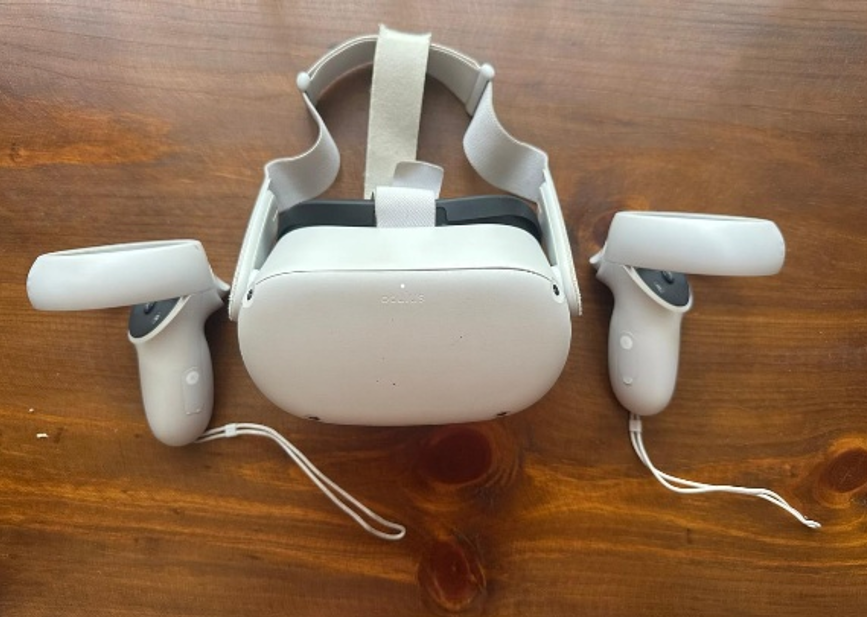
\includegraphics[width=0.65\textwidth]{imagenes/MetaQuest2}
    \caption{Visor Meta Quest 2}
    \label{fig:quest2}
\end{figure}

Para facilitar el desarrollo de aplicaciones para los dispositivos Quest, 
Meta proporciona diferentes paquetes y herramientas que conforman su 
entorno Meta XR. Dentro de Unity, Meta XR Core SDK proporciona 
funcionalidades fundamentales para el desarrollo de aplicaciones 
inmersivas y componentes específicos de la plataforma \cite{metaquestunity}.
Meta, además, proporciona además un rig XR que relaciona la 
representación de la cabeza y los dispositivos de entrada físicos con 
cámaras y elementos virtuales dentro de la escena.

En este proyecto, el Meta Quest 2 es el dispositivo utilizado para 
ejecutar y probar la experiencia en VR. Los mecanismos de entrada 
proporcionadas por el ecosistema Meta permiten obtener información de 
posición, orientación y acciones realizadas por el usuario que, 
posteriormente, puede ser interpretada por los sistemas de interacción 
implementados en Unity. De esta forma, la plataforma Meta proporciona 
la conexión entre las acciones físicas del jugador y los eventos 
utilizados por las mecánicas del videojuego.